\documentclass[a4paper]{article}
\usepackage[english,russian]{babel}
\usepackage[utf8x]{inputenc}
\usepackage[T1]{fontenc}
\usepackage[a4paper,top=2.5cm,bottom=2.5cm,left=3cm,right=1.7cm,marginparwidth=1.75cm]{geometry}
\usepackage{amsmath}
\usepackage{graphicx}
\usepackage{xcolor}
\usepackage{hyperref}
\usepackage{float}
\usepackage{indentfirst}
\usepackage{setspace}
\onehalfspacing

\usepackage[usenames,dvipsnames]{color}

\usepackage{alltt}

\usepackage{listings}
\usepackage{color}

\definecolor{dkgreen}{rgb}{0,0.6,0}
\definecolor{gray}{rgb}{0.5,0.5,0.5}
\definecolor{mauve}{rgb}{0.58,0,0.82}

\lstset{frame=tb,
  language=Octave,
  aboveskip=3mm,
  belowskip=3mm,
  showstringspaces=false,
  columns=flexible,
  basicstyle={\small\ttfamily},
  numbers=none,
  numberstyle=\tiny\color{gray},
  keywordstyle=\color{blue},
  commentstyle=\color{dkgreen},
  stringstyle=\color{mauve},
  breaklines=true,
  breakatwhitespace=true,
  tabsize=3
}

\begin{document}
% Титульны лист
\begin{titlepage}
  \begin{center}
    \large
    МИНИСТЕРСТВО ОБРАЗОВАНИЯ И НАУКИ\\ РОССИЙСКОЙ ФЕДЕРАЦИИ
     
    \textbf{Федеральное агентство по образованию}
    \vspace{0.5cm}
 
    НАЦИОНАЛЬНЫ ИССЛЕДВАТЛЬСКИЙ УНИВЕРСИТЕТ "МОСКОВСКИЙ ИНСТИТУТ ЭЛЕКТРОННОЙ ТЕХНИКИ"
    \vspace{0.25cm}
     
    Кафедра высшей математики 1
    \vfill
    
    Пономарев Александр Олегович
    \vfill
 
    \textsc{Реферат}\\[5mm]
     
    {\LARGE Решение практической задачи расчета системы \\
    охлаждения современного центрального процессора \\
    в персональном компьютере посредством \\
    системы с воздушным охлаждением}
  \bigskip
  
  3 курс, группа ПМ-31
     
\end{center}
\vfill
 
\newlength{\ML}
\settowidth{\ML}{«\underline{\hspace{0.7cm}}» \underline{\hspace{2cm}}}
\hfill\begin{minipage}{0.4\textwidth}
  Преподаватель\\
  \underline{\hspace{\ML}} М.\,А.~Гурьянов\\
  «\underline{\hspace{0.7cm}}» \underline{\hspace{2cm}} 2020 г.
\end{minipage}%
\bigskip
\vfill
 
\begin{center}
  Зеленоград, 2020 г.
\end{center}
\end{titlepage}
% Конец титульного листа

% Оглавление

\tableofcontents.

% Конец оглавления

\newpage

\section{Введение}

В данной работе решаем практическую задачу расчета системы охлаждения современного центрального процессора в персональном компьютере посредством системы с воздушным охлаждением.

Мы выбрали для себя реально существующую систему воздушного охлаждения для проведения работы и реально существующую модель центрального процессора. На основании их построили математическую модель, состоящую из уравнений теплопроводности, граничных и начальных условий. Решили их численно, рассмотрев различные варианты разностной аппроксимации линейного одномерного по пространству уравнения теплопроводности.

\newpage
\section{Выбор системы охлаждения центрального процессора}

\subsection{Выбор модели}

В качестве системы воздушного охлаждения мы выбрали систему охлаждения с тепловыми трубками: SHADOW ROCK SLIM. Он содержит в себе теплорастекательный элемент формы пластина и испарительный элемент типа стержень. 

Характеристики системы охлаждения:

\begin{itemize}
    \item Размер: 135 х 135 х 22 мм;
    \item Максимальная скорость вращения: 1400 rpm;
    \item Максимальный воздушный поток: 113.8 м3/ч;
    \item Максимальное воздушное давление: 2.1/1.23 мм водного столба;
    \item Количество тепловых трубок: 8 шт;
    \item Диаметр тепловой трубки: 6 мм;
    \item Длина трубки: 458 мм;
    \item Расстояние между пластинами: 2 мм;
    \item Ширина пластины: 0,35 мм;
\end{itemize}

\begin{figure}[h]
\center{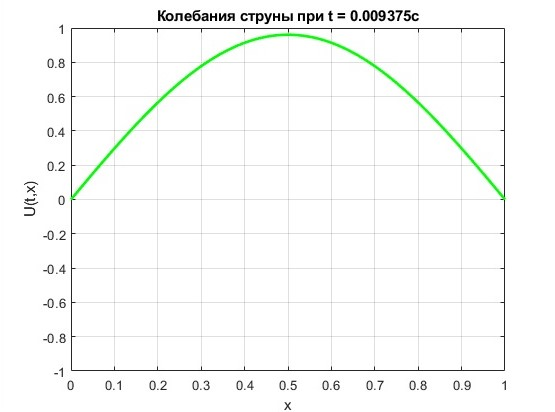
\includegraphics{1_1.png}}
\caption{Схема процессора}
\label{ris:image}
\end{figure}

Любой экземпляр данного типа можно условно разбить на группы из однотипных элементов. В данном случае это пластина (их 52 одинаковых: 52 мм (Длина) х 130 мм (Ширина) х 161 мм (Высота)) и тепловая трубка (их 8 одинаковых по 6 мм).

При этом пластину можно представить в виде прямоугольника. На пластине можно выделить точки, по которым в пластину втекает тепло (точечные источники тепла).

Стержень, с другой стороны, можно представить в виде одномерной протяженной структуры, в центре у которой расположен точечный источник тепла (процессор), а по краям расположены точки крепления к пластинам радиатора (X1…X52). Стержень, очевидно, симметричен, так что для простоты решения удобно перенести точку начала координат в точку симметрии. Результат показан на Рис. 3.

\begin{figure}[h]
\center{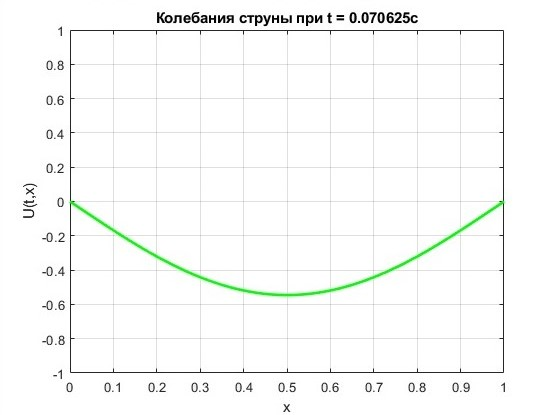
\includegraphics[scale=0.5]{1_2.jpg}}
\caption{Сеточная область пластины}
\label{ris:image}
\end{figure}

\begin{figure}[h]
\center{\includegraphics[scale=0.5]{1_33.jpg}}
\caption{Сеточная область трубки}
\label{ris:image}
\end{figure}

\newpage
\begin{center}
\begin{tabular}{ | p{100pt} | r | }
\hline
Параметр & Значение, м   \\ \hline
$l_{tube}$ & $458*10^{-3}$  \\ \hline
$l_x$ & $130*10^{-3}$   \\ \hline
$l_y$ & $52*10^{-3}$  \\ \hline
$x_1$ & $14*10^{-3}$ \\ \hline
$x_2$ & $42*10^{-3}$   \\ \hline
$x_3$ & $88*10^{-3}$   \\ \hline
$x_4$ & $113*10^{-3}$  \\ \hline
$y_1$ & $12*10^{-3}$   \\ \hline
$y_2$ & $26*10^{-3}$   \\ \hline
$X_1^{plate}...X_{52}^{plate}$ & $2*10^{-3}$ \\
\hline
\end{tabular}
\end{center}

\newpage
\section{Теоретическая постановка задачи}

\subsection{Вывод уравнения теплопроводности}

Рассмотрим физическое тело, температура которого в точке с координатами $(x, y, z)$ в момент времени t определяется функцией $u(x, y, z, t)$. Если температура различных частей тела различна, то в теле будет происходить перенос тепла от более нагретых участков тела к менее нагретым. Рассмотрим какую-нибудь поверхность $S$ внутри тела и обозначим ее малый элемент $\Delta s$. Тогда количество тепла, проходящего через элемент поверхности $\Delta s$ за время $\Delta t$, будет определяться выражением

$$\Delta Q = -k \frac{\partial u}{\partial \vec{n}}\Delta s \Delta t = -k\Delta s\Delta t \nabla_nu  \eqno(1)$$

где $k > 0$ – коэффициент теплопроводности, а $\vec{n}$ – нормаль к элементу поверхности $\Delta s$ в направлении распространения тепла. Здесь и далее $\nabla_nu = (\nabla u* \vec{n}),$ a  $\nabla u$ означает градиент функции u. Будем считать, что тело изотропно в отношении теплопроводности, т. е. коэффициент теплопроводности не зависит от направления нормали, а зависит только от координат точки. Кроме того, обозначим поток тепла через единичную площадку через $q$ т. е.

$$q=-k\frac{\partial u}{\partial \vec{n}}  \eqno(2)$$

Тогда для произвольного объема $V$ , ограниченного замкнутой поверхностью S, изменение количества тепла за промежуток времени $(t1, t2)$ будет определяться интегралом

$$Q_1= -\int\limits_{t_1}^{t^2}dt \iint\limits_S k(x,y,z) \frac{\partial u}{\partial \vec{n_0}}dS  \eqno(3)$$

где $\vec{n0}$ – внутренняя нормаль к поверхности $S$.

С другой стороны, количество тепла, необходимое для изменения
температуры выделенного объема тела на $\Delta u = u(x, y, z, t_2)−u(x, y, z, t_1)$,
равно

$$Q_2= -\int\limits_{t_1}^{t^2}dt \iiint\limits_V \rho\gamma\frac{\partial u}{\partial t}dV  \eqno(4)$$

где $\rho$ и $\gamma$ – плотность и теплоемкость данного физического тела.

Если внутри рассматриваемого тела имеются источники тепла плотности $F(x, y, z, t)$, то количество тепла, выделяемого (или поглощаемого) ими в объеме V за промежуток времени $(t_1, t_2)$, будет равно

$$Q_3= \int\limits_{t_1}^{t^2}dt \iiint\limits_V F(x,y,z,t) dV  \eqno(5)$$

Очевидно, что баланс тепла для объема $V$ определяется соотношением $Q_2 = Q_1 + Q_3$, т. е.

$$\int\limits_{t_1}^{t^2}dt \iiint\limits_V \rho\gamma\frac{\partial u}{\partial t}dV = - \int\limits_{t_1}^{t^2}dt \iint\limits_S k(x,y,z) \frac{\partial u}{\partial \vec{n_0}}dS + \int\limits_{t_1}^{t^2}dt \iiint\limits_V F(x,y,z,t) dV  \eqno(6)$$

Применяя к поверхностному интегралу формулу Гаусса-Остроградского, получим

$$\int\limits_{t_1}^{t_2}dt\iiint\limits_V \left[ \rho\gamma\frac{\partial u}{\partial t} - div(k\, grad \, u) - F(x,y,z,t)\right]  dV = 0  \eqno(7)$$

где $grad \, u = \nabla u = \frac{\partial u}{\partial x} \vec{i} + \frac{\partial u}{\partial y} \vec{j} + \frac{\partial u}{\partial z} \vec{k}$.

Так как подынтегральная функция непрерывна, а объем V и промежуток времени $(t_1, t_2)$ произвольны, то для любой точки $(x, y, z)$ и любого момента времени справедливо соотношение

$$\rho\gamma \frac{\partial u}{\partial t}=div \,(k\, grad \, u) + F(x,y,z,t) \eqno(8)$$

Это уравнение называется уравнением теплопроводности неоднородного изотропного тела. Если тело однородно, то коэффициенты $\gamma$, $\rho$, $k$ являются постоянными и уравнение теплопроводности принимает вид

$$\frac{\partial u}{\partial t} = a^2 \left( \frac{\partial^2 u}{\partial x^2} + \frac{\partial^2 u}{\partial y^2} + \frac{\partial^2 u}{\partial z^2} \right) + f(x,y,z,t) \eqno(9)$$

где $div \,(grad\,u) = \Delta u = \frac{\partial^2 u}{\partial x^2} + \frac{\partial^2 u}{\partial y^2} + \frac{\partial^2 u}{\partial z^2}$, $f(x,y,z,t)= \frac{F(x,y,z,t)}{\gamma\rho}$, $a=\sqrt{\frac{k}{\gamma\rho}}$

\subsection{Постановка начально-краевых задач для одномерного уравнения теплопроводности}

Как правило, для нахождения неизвестной функции $u(x,t)$, удовлетворяющей уравнению теплопроводности, когда пространственная переменная $x$ принадлежит некоторому интервалу $(0,l)$, а время $t$ больше нуля, необходимо задать начальное условие (при $t=0$) и краевые условия (при $x=0$, $x=l$).

Существует несколько стандартных постановок начально-краевых задач для уравнения теплопроводности на отрезке.

Математическая постановка первой начально-краевой задачи имеет вид:

$$u_t=a^2u_{xx}+f(x,t), \quad x\in(0,l), \quad t>0 \eqno(10)$$

$$u|_{t=0}=\varphi(x)$$

$$u(0,t)=\mu_1(t)$$

$$u(l,t)=\mu_2(t)$$

Здесь $u(x,t)$ подлежит определению, функции $f(x,t)$, $\varphi(x)$, $\mu_1(t)$, $\mu_2(t)$ считаются известными.

Если речь идет о процессах теплопроводности, то физическая формулировка первой краевой задачи выглядит так: найти распределение температуры $u(x,t)$ в стержне $x\in[0,l]$, если по стержню непрерывно распределены источники тепла плотности $f(x,t)$, начальное распределение температуры $\varphi(x)$ задано, на левом конце стержня температура равна $\mu_1(t)$, а на правом - $\mu_2(t)$.

Вторая краевая задача отличается от первой тем, что вместо температура на концах стержня задаются тепловые потоки:

$$-ku_x(0,t)=q_1(t)$$

$$ku_x(l,t)=q_2(t)$$


Так как коэффициент теплопроводности $k$ и величины потоков $q_1(t)$, $q_2(t)$ считаются известными, то задание потоков равносильно заданию значений первых производных функции $u(x,t)$ по переменной $x$ на концах стержня.

Полностью математическая постановка второй начально-краевой задачи выглядит так:

$$u_t=a^2u_{xx}+f(x,t), \quad x\in(0,l), \quad t>0; \eqno(11)$$

$$u|_{t=0}=\varphi(x);$$

$$u_x(0,t)=v_1(t);$$

$$u_x(l,t)=v_2(t)$$

\subsection{Численное решение уравнения теплопроводности}

Рассмотрим простейшие примеры сеток.

Пусть область изменения аргумента $x$ есть отрезок $0 \leq x \leq l$. Разобъем отрезок $0 \leq x \leq l$ точками $x_i=ih$ $(i=0,1,2...,N;h>0)$ на $N$ равных частей длины $h=\frac{l}{N}$ каждая. Множеств точек

$$x_i=ih \quad (i=0,1,2...,N;h>0)  \eqno(12)$$

называется разностной сеткой на отрезке $0 \leq x \leq l$ и обначается $\Bar{\omega}_h = {ih, i=0,1,2...,N}$, а число $h$ - расстояние между точками (узлами) cетки $\Bar{\omega}_h$ - называется шагом сетки.

Отрезок $[0,l]$ можно разбить на $N$ частей, вводя произвольные точки $x_1 \leq x_2 \leq ... \leq x_{N-1} \leq l$. Тогда получим сетку 

$$\Bar{\omega_h} = {x_i, i=0.1,...,N, \, x_0=0, \, x_N=l}  \eqno(13)$$

c шагом $h_i = x_i-x_{i-1}$, который зависит от номера $i$ узла $x_i$. Если $h_i \neq h_{i+1}$ хотя бы для дно номера $i$, то сетка $\Bar{\omega}_h = \Bar{\omega}_h^*$ называется неравномерной. Если $h_i=const=h=\frac{l}{N}$ для всех $i=1,2,...,N$, то мы получаем построенную выше равномерную сетку.

На бесконечной прямой $-\infty<x<\infty$ можно рассматривать сетку 

$$\omega_{h,x}={x+oh,i=0,\pm 1,\pm 2,... }  \eqno(14)$$

с началом в любой точке $x$, состоящую из бесконечного числа узлов.

Функцию $y_i=y(x_i)$ дискретного аргумента $x_i$, $i=0,1,...,N$, называют сеточной функцией, определенной на сетке $\overline{\omega}_h$.

Всякой непрерывной функции $f(x)$ можно поставить в соответствие сеточную функцию $f_i^h$, плагая, например, $f_i^h=f(x_i)$. Впрочем, в некоторых случаях удобнее устанавливать это соответствие другими способами.

Пусть область изменения аргументов $(x,t)$ есть прямоугольник $\Bar{D}=(0\leq x \leq 1, 0\leq t \leq T)$. Построим на отрезке $0\leq x \leq 1$ сетку $\Bar{\omega}_h={x_i=ih,i=0,1,...,N}$ с шагом $h=\frac{l}{N}$ и сетку $\Bar{\omega}_\tau={t_i=j\tau,j=0,1,...,N_0}$ с шагом $\tau=\frac{T}{N_0}$ на отрезке $0\leq t \leq T$. Множество узлов $(x_i,t_j)$ c координатами $x_i=ih$ и $t_j=j\tau$ назовем сеткой в прямоугольнике $\Bar{D}$ и обозначим 

$$\Bar{}_{h\tau}={(x_i=ih,t=j\tau), \, i=0,1,...,N, \, =0,1,...,N_0}  \eqno(15)$$

Эта сетка равноомерна по каждму и прменных $x$ и $t$. Если хотя бы дна и сетк $\Bar{\omega}_{h\tau}$ называется неравномерной. Сетка $\Bar{\omega}_{h\tau}$, очевидно, состоит из точек пересения прямых $x=x_i$, $i=0,1,...,N$ и прямых $t=t_j$, $=0,1,...,N_0$.

Пусть $y$ - сеточная функция, заданная на $\Bar{\omega}_{h\tau}$. Будем обозначать $y_i^j=y(x_i,y_j)$ значение сеточной функции $y$ в узл $x_i,t_j$ сетки $\Bar{\omega}_{h\tau}$.

Непрерывной функции $u(x,t)$, где $(x,t)$ - точка из $\Bar{D}$, будм ставить в соответствие сеточную функцию 

$$u_i^j=u_{i,h,\tau}^j=u(x_i,t_j)  \eqno(16)$$

\subsection{Явная схема}

Уравнение теплопроводности:

$$\frac{\partial u}{\partial t} = \frac{\partial^2 u}{\partial x^2} +f(x,t), \, x\in(0,l), \, t\in(0,T] \eqno(17)$$

Для аппроксимации оператора $L=\frac{\partial}{\partial t}-\frac{\partial^2}{\partial x^2}$ в уравнении (17) используем шаблон, приведенный на рис.4

\begin{figure}[h]
\center{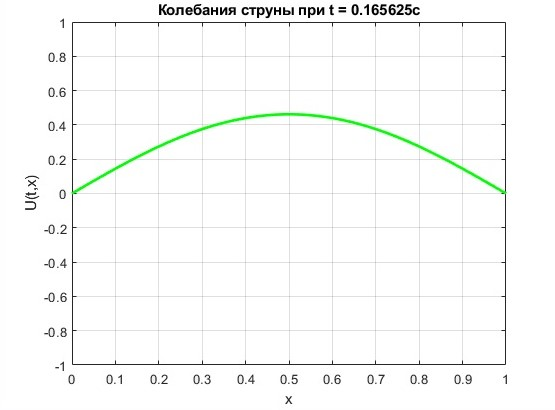
\includegraphics[scale=0.3]{1_3.png}}
\caption{Шаблон явной схемы для уравнения теплопроводности}
\label{ris:image}
\end{figure}

Соответствующий разностный оператор $L_{h\tau}^{(0)}u$ и имеет вид:

$$L_{h\tau}^{(0)}u=\frac{u(x,t)+\tau-u(x,t)}{\tau}-\frac{u(x+h,t)-2u(x,t)+u(x-h,t)}{h^2} \eqno(18)$$

Далее для кратности будем использовать следующие стандартные обозначения:

$$u=u(x,t); \quad  u^{*}=u(x,t+\tau)$$

Тогда:

$$u_t=\frac{u^{*}-u}{\tau}, \quad L_{h\tau}^{(0)}u=u_t-u_{\Bar{x}x}$$

Найдем погрешность аппроксимации разностным оператором $L_{h\tau}^{(0)}$ исходного дифференциального оператора $L$ в точке $(x, t)$. В случае достаточно гладкой функции $u(x, t)$ при достаточно малых шагах $h$ и $\tau$ имеем:

$$u_t=\frac{u(x,t+\tau)-u(x,t)}{\tau}=\frac{\partial u(x,t)}{\partial t}+O(\tau) \eqno(19)$$

$$u_{\Bar{x}x}=\frac{\partial^2u(x,t)}{\partial x^2}+O(h^2)  \eqno(20)$$

Следовательно, разностный оператор $L^{(0)}_{h\tau}$ аппроксимирует дифференциальный оператор $L$ с погрешностью $O(\tau + h^2)$ в точке $(x, t)$:

$$L^{(0)}_{h\tau}u=\underbrace{\frac{\partial u(x,t)}{\partial t}-\frac{\partial^2u(x,t)}{\partial x^2}}_{L[u(x,t)]} + O(\tau+h^2)  \eqno(21)$$

Введем сеточную функцию $\phi = \varphi(x_i, t_j )$, аппроксимирующую правую часть $f(x, t)$ уравнения (17) на всех внутренних узлах $(x_i, t_j )$ сетки с погрешностью $O(\tau + h_2)$. В качестве $\varphi$ можно взять, например $\varphi(x_i, t_j ) = f(x_i, t_j )$. Тогда разностное уравнение

$$L_{h\tau}^{(0)}y=\varphi  \eqno(22)$$

будет аппроксимировать исходное дифференциальное уравнение теплопроводности (17) с
первым порядком погрешности по $\tau$ и вторым по $h$.

\subsection{Неявная схема}

Используем для аппроксимации оператора $L=\frac{\partial}{\partial t} - \frac{\partial^2}{\partial x^2}$ в уравнении (17) шаблон, приведенный на Рис.5

\begin{figure}[h]
\center{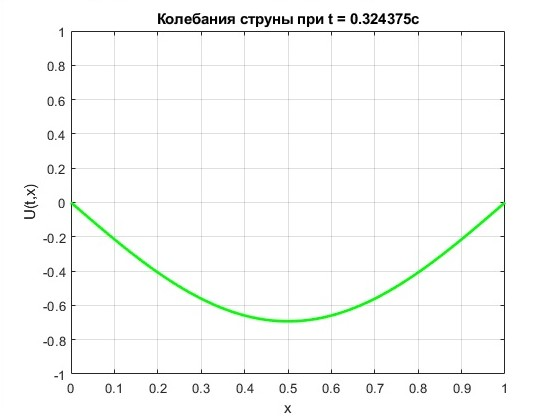
\includegraphics[scale=0.3]{1_4.png}}
\caption{Шаблон ytявной схемы для уравнения теплопроводности}
\label{ris:image}
\end{figure}

Тогда разностная аппроксимация оператора $L$ уравнения теплопроводности будет выглядеть следующим образом:

$$L_{h\tau}^{(1)}u=\frac{u(x,t+\tau)-u(x,t)}{\tau}-\frac{u(x+h,t+\tau)-2u(x,t+\tau)+u(x-h,t+\tau)}{h^2}=u_t-u_{\Bar{x}x}^{*} \eqno(23)$$

Рассмотрим погрешность аппроксимации разностным оператором $L^{(1)}_{h\tau}$ исходного дифференциального оператора $L$ в точках $(x, t)$, $(x, t + \tau)$. Так как для достаточно гладкой функции $u(x, t)$ справедливы равенства

$$u_{\Bar{x}x}^{*}=\frac{\partial^2u(x,t+\tau)}{\partial x^2} +O(h^2) = \frac{\partial^2u(x,t)}{\partial x^2}+O(\tau+h^2)  \eqno(24)$$

то с учетом (19) получаем, что оператор $L^{(1)}_{h\tau}$ аппроксимирует дифференциальный оператор $L$ в уравнении (17) с погрешностью $O(\tau + h^2)$ в точках $(x, t)$ и $(x,t+\tau)$:

$$L^{(1)}_{h\tau}u = \frac{\partial u(x,t)}{\partial t} +O(\tau) - \frac{\partial^2u(x,t)}{\partial x^2} +O(\tau+h^2) = \underbrace{\frac{\partial u(x,t)}{\partial t} - \frac{\partial^2u(x,t)}{\partial x^2}}_{L[u(x,t)]} +O(\tau+h^2) \eqno(25)$$

$$L^{(1)}_{h\tau}u = \frac{\partial u(x,t+\tau)}{\partial t} +O(\tau) - \frac{\partial^2u(x,t+\tau)}{\partial x^2} +O(h^2) = \underbrace{\frac{\partial u(x,t+\tau)}{\partial t} - \frac{\partial^2u(x,t+\tau)}{\partial x^2}}_{L[u(x,t+\tau)]} +O(\tau+h^2) \eqno(26)$$

Беря в качестве сеточной аппроксимации правой части уравнения (15), например, функцию $\varphi(x_i, t_j ) = f(x_i, t_{j+1})$, получим разностное уравнение

$$L_{h\tau}^{(1)}y=\varphi \eqno(27)$$

аппроксимирующее (17) с погрешностью $O(\tau + h^2)$.

\newpage
\section{Практическая построение математической модели}

\subsection{Построение математической модели}

При построении математической модели нужно учитывать следующие вещи:

Для пластины:

\begin{enumerate}
    \item Коэффициент $a$ опрделяется материалом
    \item Чем горячее пластина, тем больше скорость теплоотдачи
    \item Функции равна нулю везде кроме $x=x_j$
    \item Кулер пытается охладить пластину
    \item Теплоперенос пропорционален разнице температур
    \item Коеффициент теплопроводности зависимост от способа крепления пластин
    \item Температура в комнате $+24^oC$
    \item На границах пластины отсутствует теплообмен
    \item Охлаждение пропорционально скорости вращения кулера
\end{enumerate}

Теперь адптируем дифференциальное уравнение теплопроводности:

$$V_t=a^2V_{xx}-\sum\limits_{x_j}\sigma(x-x_j)*k*(V(x_j,t)-U_j)-F \eqno(28)$$

$$F=r*RPM$$

$$V'(0,t)=0$$

$$V'(l,t)=0$$

$$V(x,0)=24$$

Для стержня:

\begin{enumerate}
    \item Коэффициент $a$ определяется материалом
    \item Чем горячее стержень, тем больше скорость теплоотдачи
    \item Функции равна нулю везде кроме $x=x_i$
    \item Теплоперенос пропорционален разнице температур
    \item Коэффициент теплопроводности зависит от способа крепления пластин
    \item Температура в комнате $+24^oC$
    \item В другом конце стержня движение тепла  отсутствует
    \item В начале стержня непрерывный источник тепла
\end{enumerate}

Теперь адптируем дифференциальное уравнение теплопроводности:

$$U_t=a^2U_{xx}-\sum\limits_{x_i}\sigma(x-x_i)*k*(U(x_i,t)-V_i)  \eqno(29)$$

$$U'(0,t)=+p/4$$

$$U'(l,t)=0$$

$$U(x,0)=24$$

Перейдем к составлению математической модели системы охлаждения современного центрального процессора:

Краевая задача 1:

$$U'_{j_t}(x_n,t_m)=a^2U''_{j_{xx}}(x_n,t_m)-\sum\limits_{x_i}\sigma(x_n-x_i)*k*(U_j(x_n,t_{m-1}-V_i(x_i^v,t_{m-1}))  \eqno(30)$$

$$U'_j(0,t)=+p/4$$

$$U'_j(l,t)=0$$

$$U_j(x,0)=24$$

$$x_n=x\times dx, \quad n\in\left[ 1, \frac{l}{dx} \right]$$

$$t_m=m\times dt, \quad  m\in\mathbb{N}$$

$$j=1,2,...,8$$

$$j=1,2,...,52$$

Краевая задача 2:

$$V'_{i_t}(x_n,t_m)=a^2V''_{i_{xx}}(x_n,t_m)-\sum\limits_{x_j}\sigma(x_n-x_j)*k*(V_i(x_n,t_{m-1})-U_j(x_n^U,t_{m-1}))-F  \eqno(31)$$

$$F=r*RPM$$

$$V'(0,t)=0$$

$$V'(l,t)=0$$

$$V(x,0)=24$$

$$x_n=x\times dx, \quad n\in\left[ 1, \frac{l}{dx} \right]$$

$$t_m=m\times dt, \quad  m\in\mathbb{N}$$

$$j=1,2,...,8$$

$$j=1,2,...,52$$

\subsection{Факторы внешней среды}

Теперь необходимо описать внешние условия:

Для задачи 1 (Стержень) факторами внешней среды (правая часть уравнения) будут:
Тепло передаваемое процессором (Граничное условие №1 следовательно будет источником тепла)
тепло отнимаемое пластинами – Задача 1 и задача 2 связаны.

Для задачи 2 (Пластина) факторами внешней (правая часть уравнения) среды будут:
тепло.

\subsection{Недостатки математичкой модели}

\begin{enumerate}
    \item Не учитываем толщину пластины. \\
    Верхня и нижняя грань в реальности будут иметь разную температуру, так как тепло передается внутри пластины не мгновенно.Также при изготовлении металических пластин, если оборудованние на заводе изношенно, то пластины получатся с подогнутыми краями, и воздух будет скапливаться за преградами, так как там зона пониженного давления. 
    \item Для одномерного случая не учитывается ширина пластин. \\
    Так как скорость передачи тепла внутри пластины не бесконечно большая, пластина в трехмерном случае будет иметь разную температуру в каждой точке пластины, что наша модель не учитывает.
    \item Мы не учитываем толщину стержня и рассматриваем его, как одномерный случай.
    \item Не учитываем турбулентность и охлаждение пластин и трубок окружающей средой. \\
    Но его толщиной можно пренебречь, потому что охлаждение окружающей средой на порядки меньше чем охлаждение куллером.
    \item Математическая модель не учитывает того, что коэффициент теплопроводности, удельная теплоемкость и плотность зависят от температуры.

\end{enumerate}

\newpage
\section{Моделирование средствами MATLAB}

\subsection{Реализация явной схемы}

Рассмотрим начально-краевую задачу на отрезке $x\in [0,l]$:


$$\left\{
\begin{aligned}
\frac{\partial u}{\partial t}=a^2\frac{\partial^2 u}{\partial x^2}+f \\
u(x,0)=24 \\
u'(0,t)=0 \\
u'(0,l)=0
\end{aligned}
\right.$$

Для того, чтобы получить численное решение, введем в расчетной области равномерную сетку:

$$x_n=nh, \quad n=0,1,...,N, \quad hN=l, \quad t_j=j\tau, \quad j=0,1,...,J, \quad \tau J=l \eqno(32)$$
такую что $\tau\leq h^2/2$. Для этого достаточно $N$ задать произвольно, а $J$ выбрать так, чтобы выполнялось неравенство $J\geq2N^2$.

Построим разностную аппроксимацию уравнения в соответствии с явной схемой:

$$\frac{y_n^{j+1}-y_n^j}{\tau}=\frac{y_{n-1}^j-2y_n^j+y_{n+1}^j}{h^2}+f_n, \quad n=1,2,...,N-1, \quad j=0,1,...,J-1 \eqno(33)$$

Это разностное уравнение необходимо дополнить соответствующими начальными и
граничными условиями на сетке. Начальное условие и граничное условие второго рода аппроксимируются точно:

$$y_n^0=24$$

Граничное условие при $x = 1$ содержит производную $\frac{\partial u}{\partial x}$. Если ее просто заменить односторонней разностной производной, то уравнение

$$\frac{y_N^j-y_{N-1}^j}{h}=0, \quad j=0,1,...,J \eqno(34)$$
$$\frac{y_2^j-y_1^j}{h}=0, \quad j=0,1,...,J \eqno(35)$$
будет аппроксимировать соответствующее граничное условие с первым порядком погрешности аппроксимации по h. Это означает, что и для всей разностной схемы порядок погрешности аппроксимации по h будет первым.

Для того, чтобы для всей схемы сохранить погрешность аппроксимации $O(\tau) + O(h^2)$, можно использовать различные подходы. Например, можно аппроксимировать граничное условие с помощью трехточечной односторонней производной.

В результате получим следующую разностную схему:

$$\begin{cases}
\frac{y_n^{j+1-y_n^j}}{\tau}=\frac{y_{n-1}^j-2y_n^j+y_{n+1}^1}{h^2}+f_n, \quad n=1,...,N-1, \quad j=0,...,J-1\\
\frac{-3y_0^{j+1}+4y_1^j{j+1}-y_2^{j+1}}{2h}=0; \quad \frac{3y_N^{j+1}-4y_{N-1}^j{j+1}-y_{N-2}^{j+1}}{2h}=0 , \quad n=1,...,N-1, \quad j=0,...,J-1\\
y_n^0=24, \quad n=0,1,...,N 
 \end{cases}$$

Рассмотрим алгоритм решения этой системы. При j = 0 значения $y^0_n$ известны из начального условия, а значения $y^1_n$ неизвестны и должны быть найдены для всех $n=0, 1, ..., N$. Когда найдены все значения $y^1_n$, нужно найти $y^2_n$ и т.д. Следовательно, при каждом фиксированном $j = 0, 1, ..., J − 1$ неизвестными являются значения $y^{j+1}_n$. Найти их можно следующим образом:

1) При $n=1,2,...,N-1$ из (1):

$$y_n^{j+1}=y_n^j+\frac{\tau}{h^2}(y_{n+1}^j-2y_n^j+y_{n-1}^j)+\tau f_n \eqno(36)$$

2) При $n=0$ и $n=N$:

$$y_0^{j+1}=\frac{4}{3}y_1^{j+1}-\frac{1}{3}y_2^{j+1} \eqno(37)$$

$$y_N^{j+1}=\frac{4}{3}y_{N-1}^{j+1}-\frac{1}{3}y_{N-2}^{j+1} \eqno(38)$$

3) Переходим на новый слой по времени, увеличивая $j$ на единицу и повторяем действия 1) и 2).

\subsection{Визуализация в MATLAB}

Для визуального представлениям явной схемы смоделируем подзадачу похожую на нашу краевую задачу с пластиной. Отличие будем в том, что передавать будут не стержни, а некоторая функция в специальных точках для наглядности.

Возьмем пластину единичной длины и разобьем ее на некоторые элементарные участки. И на те участки, которые кратны 5, 6 и 7 будем передавать значения нашей функции, но без охлаждения для того, чтобы проследить теплопередачу от стрежня к пластине. Естественно, зададим начальную температуру $24^oC$:

\lstinputlisting{visual.m}

\begin{figure}[h]
\begin{center}
\begin{minipage}[h]{0.4\linewidth}
\includegraphics[width=1\linewidth]{1_5.png}
\caption{} %% подпись к рисунку
\label{ris:experimoriginal}
\end{minipage}
\hfill
\begin{minipage}[h]{0.4\linewidth}
\includegraphics[width=1\linewidth]{1_6.png}
\caption{}
\label{ris:experimcoded}
\end{minipage}
\end{center}
\end{figure}

На графике видно, что значения смещаются к концу пластины. Это происходит из-за того, что мы запускаем итерационный процесс от $0$ к $l$, при этом в соответствии с исходной задачей у нас граничные условия второго рода:$V'(0,t)=0$, $V'(l,t)=0$, что говорит о том, что теплопотери на концах нулевые, из-за чего и происходит смещение.

\newpage
\section{Моделирование двумерного случая средствами MATLAB}

\subsection{Вывод сеточной функции для двумерного случая}

Рассмотрим решения уравнений параболического типа рассмотрим нестационарное уравнение теплопроводности

$$\rho(x,y)X(x,y)\frac{\partial T}{\partial t}-\Delta(k(x,y)\Delta T)=f(x,y)  \eqno(38)$$
где $t$ – время; $x$, $y$ – координаты; $T(x, y)$ – искомая функция распределения абсолютной температуры по координатам; $\rho(x, y)$ – плотность вещества; $C(x, y)$ – удельная теплоемкость вещества; $k(x, y)$ – коэффициент теплопроводности вещества; $f(x, y)$ – плотность мощности источников тепла на прямоугольной области с граничными условиями Дирихле или Неймана на границах $x = x_{min}$, $x = x_{max}$, $y = y_{min}$, $y = y_{max}$ и начальными условиями первого или второгорода н8а отрезке времени $[t_{min}, t_{max}]$. Зададим на отрезке $[x_{min}, x_{max}]$ равномерную координатную сетку с шагом $\Delta x$:

$$x={x_i|i=1,2,...,n}  \eqno(40)$$
на отрезке $y_{min},y_{max}$ -- равномерную координатную сетку с шагом $\Delta y$:

$$y={y_j|j=1,2...,m} \eqno(41)$$
на отрезке $t_{min},t_{max}$ -- равномерную координатную сетку с шагом $\Delta t$:

$$y={t_l|l=1,2...,s}  \eqno(42)$$

Векторы, заданные выражениями (40) – (42), определяют на прямоугольной области равномерную пространственно-временную сетку:

$$G={x_i,y_j,t_l|i=1,2,...,n,j=1,2,...,m,t=1,2,...,s} \eqno(43)$$

Граничные условия второго рода (Неймана) для рассматриваемой задачи могут быть представлены в виде:

$$\frac{\partial T}{\partial x}\bigg|_{x_1,y,t}=g_1(y)  \eqno(44)$$

$$\frac{\partial T}{\partial x}\bigg|_{x_n,y,t}=g_2(y)  \eqno(45)$$

$$\frac{\partial T}{\partial y}\bigg|_{x,y_1,t}=g_3(y)  \eqno(46)$$

$$\frac{\partial T}{\partial y}\bigg|_{x,y_n,t}=g_4(y)  \eqno(47)$$

Начальные условия первого рода для рассматриваемой задачи могут быть представлены в виде:

$$T(x,y,t_1)=g_t(x,y) \eqno(48)$$
где $t_1$ - начальный момент времени; $g_t(x,y)$ некоторая непрерывная функция соответствующих координат.

\subsection{Реализация в MATLAB}

Рассмотриим реализацию двумерного уравнения теплопроводности на языке MATLAB.

\lstinputlisting{heatEquation2D.m}

Результат работы скрипта:

\begin{figure}[h]
\begin{center}
\begin{minipage}[h]{0.4\linewidth}
\includegraphics[width=1\linewidth]{11_6.jpg}
\caption{} %% подпись к рисунку
\label{ris:experimoriginal}
\end{minipage}
\hfill
\begin{minipage}[h]{0.4\linewidth}
\includegraphics[width=1\linewidth]{11_5.jpg}
\caption{}
\label{ris:experimcoded}
\end{minipage}
\end{center}
\end{figure}

\begin{figure}[h]
\begin{center}
\begin{minipage}[h]{0.4\linewidth}
\includegraphics[width=1\linewidth]{11_4.jpg}
\caption{} %% подпись к рисунку
\label{ris:experimoriginal}
\end{minipage}
\hfill
\begin{minipage}[h]{0.4\linewidth}
\includegraphics[width=1\linewidth]{11_3.jpg}
\caption{}
\label{ris:experimcoded}
\end{minipage}
\end{center}
\end{figure}

\begin{figure}[H]
\begin{center}
\begin{minipage}[h]{0.4\linewidth}
\includegraphics[width=1\linewidth]{11_2.jpg}
\caption{} %% подпись к рисунку
\label{ris:experimoriginal}
\end{minipage}
\hfill
\begin{minipage}[h]{0.4\linewidth}
\includegraphics[width=1\linewidth]{11_1.jpg}
\caption{}
\label{ris:experimcoded}
\end{minipage}
\end{center}
\end{figure}


\newpage
\section{Решение в MATALAB и проверка}

\subsection{Реализация}

Результируя все выводы полученные выше, реализуем код в MATALAB:

\lstinputlisting{explicit1_mat_model.m.m}

При $ t = 1 сек $ получили графики:

\begin{figure}[H]
\begin{center}
\begin{minipage}[h]{0.4\linewidth}
\includegraphics[width=1\linewidth]{1_7.png}
\caption{} %% подпись к рисунку
\label{ris:experimoriginal}
\end{minipage}
\hfill
\begin{minipage}[h]{0.4\linewidth}
\includegraphics[width=1\linewidth]{1_8.png}
\caption{}
\label{ris:experimcoded}
\end{minipage}
\end{center}
\end{figure}

\begin{figure}[H]
\begin{center}
\begin{minipage}[h]{0.4\linewidth}
\includegraphics[width=1\linewidth]{1_9.png}
\caption{} %% подпись к рисунку
\label{ris:experimoriginal}
\end{minipage}
\hfill
\begin{minipage}[h]{0.4\linewidth}
\includegraphics[width=1\linewidth]{1_10.png}
\caption{}
\label{ris:experimcoded}
\end{minipage}
\end{center}
\end{figure}

При $t=10 сек$ получили графики:

\begin{figure}[H]
\begin{center}
\begin{minipage}[h]{0.4\linewidth}
\includegraphics[width=1\linewidth]{1_11.png}
\caption{} %% подпись к рисунку
\label{ris:experimoriginal}
\end{minipage}
\hfill
\begin{minipage}[h]{0.4\linewidth}
\includegraphics[width=1\linewidth]{1_12.png}
\caption{}
\label{ris:experimcoded}
\end{minipage}
\end{center}
\end{figure}

\begin{figure}[H]
\begin{center}
\begin{minipage}[h]{0.4\linewidth}
\includegraphics[width=1\linewidth]{1_13.png}
\caption{} %% подпись к рисунку
\label{ris:experimoriginal}
\end{minipage}
\hfill
\begin{minipage}[h]{0.4\linewidth}
\includegraphics[width=1\linewidth]{1_14.png}
\caption{}
\label{ris:experimcoded}
\end{minipage}
\end{center}
\end{figure}

\subsection{Тесты}

Наша конфигурация:

\begin{enumerate}
    \item Processor - Intel Core i7-3930K
    \item Motherboard - Gigabyte X79-UP4
    \item Memory - 8GB Corsair Vengeance LP 1600MHz CL9
    \item Video Card - Sapphire Radeon HD 6850 1GB
    \item Power Supply - NZXT Hale90 650W
    \item Storage Drive - Kingston HyperX 240GB SATA III SSD
    \item Case - Corsair Carbide 760T
    \item Monitor ASUS ROG SWIFT PG278Q
    \item The system used is as follows and tests are performed 4.4 GHz frequencies
\end{enumerate}

\begin{figure}[H]
\center{\includegraphics[scale=0.5]{test_1.png}}
\caption{Устоявшаяся температура}
\label{ris:image}
\end{figure}

\newpage
\section{Вывод}

Мы рассмотрели математическую модель системы охлаждения центрального процессора, разбив ее на составляющиее компоненты, а именно: трубки и пластины. Данная математическая модель имеет ряд недостатков, описанные в нашей работе, но несмотря на это, мы смогли получить достаточно точный результат, описывающий данную систему. Расхождение составило порядка $5-6^oC$, что является неплохим результатом, учитывая наши грубые предположения.

% Ссылки
\newpage

\begin{thebibliography}{9}
\bibitem .В.В. Лесин учебное пособие "Уравнение математической физики"
\bibitem \href{https://www.bequiet.com/en/cpucooler/479}
\bibitem \href{https://www.kitguru.net/components/silas-newman/be-quiet-dark-rock-slim-review/5/}
\bibitem \href{http://www.mmcs.sfedu.ru/jdownload/finish/16-kafedra-vychislitelnoj-matematiki-i-matematicheskoj-fiziki/1419-uravneniya-matematicheskoj-fiziki-zadachi-i-resheniya-s-v-revina-l-i-sazonov-o-a-tsyvenkova}
\bibitem \href{https://www.vortez.net/articles\_pages/be\_quiet\_dark\_rock\_slim\_review,7.html}

\end{thebibliography}

\end{document}
